\section{Experiments}
\label{sec:exp}
In this section we first introduce the popular ATIS dataset\footnote{ \url{https://github.com/yvchen/JointSLU/tree/master/data}},
then describe how we collect our \textbf{E}-\textbf{c}ommerce \textbf{S}hopping \textbf{A}ssistant (ECSA) dataset\footnote{ \url{https://github.com/pangolulu/DCMTL}}.
Then we show the implementation details for our model.
Finally we demonstrate the evaluation results on both ATIS and ECSA dataset and give some discussions.
In the following experiments, we call our proposed \textbf{D}eep \textbf{C}ascade \textbf{M}ulti-\textbf{T}ask \textbf{L}earning method as DCMTL for short.

\subsection{Dataset}
\label{sec:data}
%\noindent
\subsubsection{ATIS Dataset}
The ATIS corpus, the most commonly used dataset for slot filling research, contains reservation requests for air travel.
It contains 4,978 training and 893 testing sentences in total, with a vocabulary size of 572 \cite{mesnil2015using}. 
%We randomly selected 80\% of the training data for model training and the rest 20\% as the validation set  \cite{mesnil2015using}.
Apart from the ground-truth slot labels, we also generate its 
corresponding segment labels for our multi-task model setting.

%\noindent
\subsubsection{ECSA Dataset}
\label{sec:ECSGA_data}
To create large amounts of gold standard data 
to train our model,
we adopt an unsupervised method to 
automatically tag the input utterances.
All the utterances are extracted from the user input logs 
(either from text or voice) on our online shopping 
assistant system. Besides our E-commerce knowledge-base
is a dictionary consisting of pairs of
word terms and their ground-truth slot labels 
such as ``red-\textbf{Color}'' or ``Nike-\textbf{Brand}''.
Since this resource is created by human beings,
we will use it to create gold standard.
We use a dynamic programming algorithm of max-matching to 
match words in the utterances and then assign each word with 
its slot label in IOB scheme.
We filter utterances whose matching result is
ambiguous and only reserve those that can be 
perfectly matched
(all words can be tagged by only one unique label) 
as our training and testing data.
With the slot labels of each word, we can induce the 
named entity labels and segment labels straightforwardly via the E-commerce knowledge-base.
For we only extract the perfectly matched sentences,
the quality of our ECSA dataset can be guaranteed.
It can be considered as a long-distance supervision method \cite{mintz2009distant}.
%Our goal is to develop 
%One may wonder why we can't just use the max-matching algorithm and 
%a good dictionary to do the slot filling itself.
%However the dictionary can only cover or recognize limited sentences.
%a sequence labeling algorithm with the ability to generalize to vocabulary
%outside of the dictionary.
%In fact, for our online usage we first use a dictionary to apply max-matching algorithm to do tagging,
%and if we cannot tag the input sentence perfectly we will adopt our trained model to do inference.
%This is just for the concern of online efficiency.

To evaluate model's ability to generalize, 
we randomly split the dictionary into three parts.
%For the balance concern of each slot label occurring in 
%the training and testing dataset,
%we split the dictionary according to the dimension of slot labels.
%Finally
One part is used to generate testing data and the other two 
to generate training data.
If we don't split the dictionary and use the whole to generate 
both training and testing data,
then the trained model may remember the whole dictionary and 
the results will not reflect the true performance of the models.

This unsupervised approach 
alleviates human annotations, 
and we can produce a large volume of labeled data automatically. 
The following experiments use a dataset of 24,892 training pairs
and 2,723 testing pairs.
Each pair contains an input utterance $\bi{w}$, 
its corresponding gold sequence of slot labels $\bi{y}^{slot}$,
named entity labels $\bi{y}^{ne}$ and segment labels $\bi{y}^{seg}$.
The vocabulary size of ECSA is 1265 (Chinese characters), and the amount of segmented terms can be much larger.
The Out-of-Vocabulary (OOV) rate of ESCA dataset is 85.3\% (Meaning 85.3\% of terms in testing data never appear in training data) while the OOV rate of ATIS is lower than 1\%.
Apparently slot filling task on ESCA dataset is more challenging. 

\subsection{Implementation Details}
\label{sec:implementation}
For the RNN component in our system,
we use a 3-layers BiLSTM networks for ECSA and 2-layers BiLSTM networks for ATIS (no named entity tagging in this case),
and all LSTM networks come with hidden state size 100.
%All input sentences are padded to a maximum sequence length of 21 in ECSA dataset and 46 in ATIS dataset.
The input in ECSA is a sequence of Chinese characters rather that words 
since there is no segmentation.
The dimension of embedding layer $E$ 
and BiLSTM network output state (concatenation of the forward and backward LSTM) are set to 200.
%For experiments on ECSA dataset, the size of the labels for slot filling,
%named entity tagging and segment tagging are 57, 7 and 3 respectively.
%For experiments on ATIS dataset, the size of the labels for slot filling and 
%segment tagging are 127 and 3 (no named entity tagging in this case).
%The vocabulary sizes of ECSA and ATIS dataset are 1265 and 572 respectively.
We perform a mini-batch log-likelihood loss training with a batch size of 
32 sentences for 10 training epochs.
We use Adam optimizer, and the learning rate is initialized to 0.001.
To prevent the gradient explosion problem for training LSTM networks,
we set gradient clip-norm as 5.

\subsection{Results and Discussions}
\label{sec:eval}

%\noindent
\subsubsection{Evaluation on ATIS}
We compare the ATIS results of our DCMTL model with current published results in \tabref{tab:eval_ATIS}.
%{\color{red}[[Modification Start]]}
We split the methods into two categories:
one is \emph{Sequence Labeling} based method, and the other is \emph{Encoder-Decoder} based method.
Sequence Labeling based method generally adopts a sequential network
(RNN \cite{yao2013recurrent,yao2014spoken,liu2015recurrent,peng2015recurrent,vu2016bi} or CNN \cite{xu2013convolutional,vu2016sequential})
and calculate a loss function (such as CRF loss \cite{xu2013convolutional}, cross entropy loss \cite{yao2013recurrent,yao2014spoken} or ranking loss \cite{vu2016bi}) on top of the network output.
Encoder-Decoder based method, on the other hand, 
usually employs a RNN to encode the whole sentence 
and another RNN to decode the labels \cite{kurata2016leveraging}.
The decoder will attend to the whole encoding sequence with attention mechanism \cite{zhu2017encoder,zhai2017neural}.
Our method follows the Sequence Labeling framework 
and we design a novel multi-task sequence labeling model
which achieve the best performance against the published Sequence Labeling based method (F1+0.22\%)
and compatible result against the best Encoder-Decoder based method (F1-0.03\%).
As we claim in \secref{sec:intro}, 
more than 97\% of chunks in ATIS dataset have only one or two words and there are no named entity labels at all.
These two reasons prevent our proposed DCMTL model from further improving the performance on ATIS dataset.
Thus, we will mainly focus on ECSA dataset, 
which is much larger and more sophisticated,
to prove the effectiveness of our proposed model.
%{\color{red}[[Modification End]]}

%most of works use deep neural networks for slot filling.
Besides, almost all the methods (including ours) 
reach very high F1 score of around 0.96.
%Our result is the second highest.
This also makes us wonder
whether it is meaningful enough to continue evaluating on this dataset,
for minor differences in the results may be attributed to data variance
more than the models.
Apparently high performance on ATIS does not 
mean working on real-world application
which contains more informative semantic slot labels and more complicated 
expressions as in the case of online shopping assistant.
\begin{table}[th]
	\centering
	\scriptsize
	\begin{tabular}{c|c}
		\toprule
		Methods & F1 \\
		\midrule
		simple RNN \cite{yao2013recurrent} & 0.9411 \\
		CNN-CRF \cite{xu2013convolutional} & 0.9435 \\
		LSTM \cite{yao2014spoken} & 0.9485 \\
		RNN-SOP \cite{liu2015recurrent} & 0.9489 \\
		Deep LSTM \cite{yao2014spoken} & 0.9508 \\
		RNN-EM \cite{peng2015recurrent} & 0.9525 \\
		Bi-RNN with ranking loss \cite{vu2016bi} & 0.9547 \\
		Sequential CNN  \cite{vu2016sequential} & \underline{0.9561} \\
		\midrule
		Encoder-labeler Deep LSTM \cite{kurata2016leveraging} & 0.9566 \\
		BiLSTM-LSTM (focus) \cite{zhu2017encoder} & 0.9579 \\
		Neural Sequence Chunking \cite{zhai2017neural} & \textbf{0.9586} \\
		\midrule
		DCMTL (Ours) & $\underline{0.9583}^{*}$  \\
		\bottomrule
	\end{tabular}
	\caption{Comparison with published results on the ATIS dataset.}
	\label{tab:eval_ATIS}
	%\vspace{-10pt}
\end{table}

%\noindent
\subsubsection{Evaluation on ECSA}
\begin{table}[th]
	\centering
	\scriptsize
	\begin{tabular}{c|ccc}
		\toprule
		Models & Precision & Recall & F1 \\
		\midrule
		Basic BiLSTM-CRF & 0.4330 & 0.4275 & 0.4302 \\
		* Basic BiLSTM-CRF (cond. SEG) & 0.7948 & 0.7953 & 0.7950 \\
		* Basic BiLSTM-CRF (cond. NE) & 0.8985 & 0.8986 & 0.8985 \\
		\midrule
		Vanilla Multi-task & 0.3990 & 0.3941 & 0.3965 \\
		Hierarchy Multi-task & 0.4417 & 0.4494 & 0.4455 \\
		%\midrule
		%Sequential CNN  \cite{vu2016sequential} & 0.xxxx & 0.xxxx & 0.2877 \\
		%Neural Sequence Chunking \cite{zhai2017neural} & 0.xxxx & 0.xxxx & 0.xxxx \\
		\midrule
		** DCMTL (\textbf{-} cascade) & 0.4654  & 0.4613 & 0.4633  \\
		** DCMTL (\textbf{-} residual) & 0.4923 & 0.4760 & 0.4840  \\
		DCMTL (full) & \textbf{0.5281} & \textbf{0.4941} & \textbf{0.5105} \\
		\bottomrule
	\end{tabular}
	\caption{Results for slot filling task on the ECSA dataset.
		Columns with highlighted boldface are the best performance.
		Rows with * prefix are just results for our case study.
		Rows with ** prefix are results for ablation test.}
	\label{tab:eval_ECSGA}
	%\vspace{-10pt}
\end{table}

\begin{figure}[h]
	\centering
	%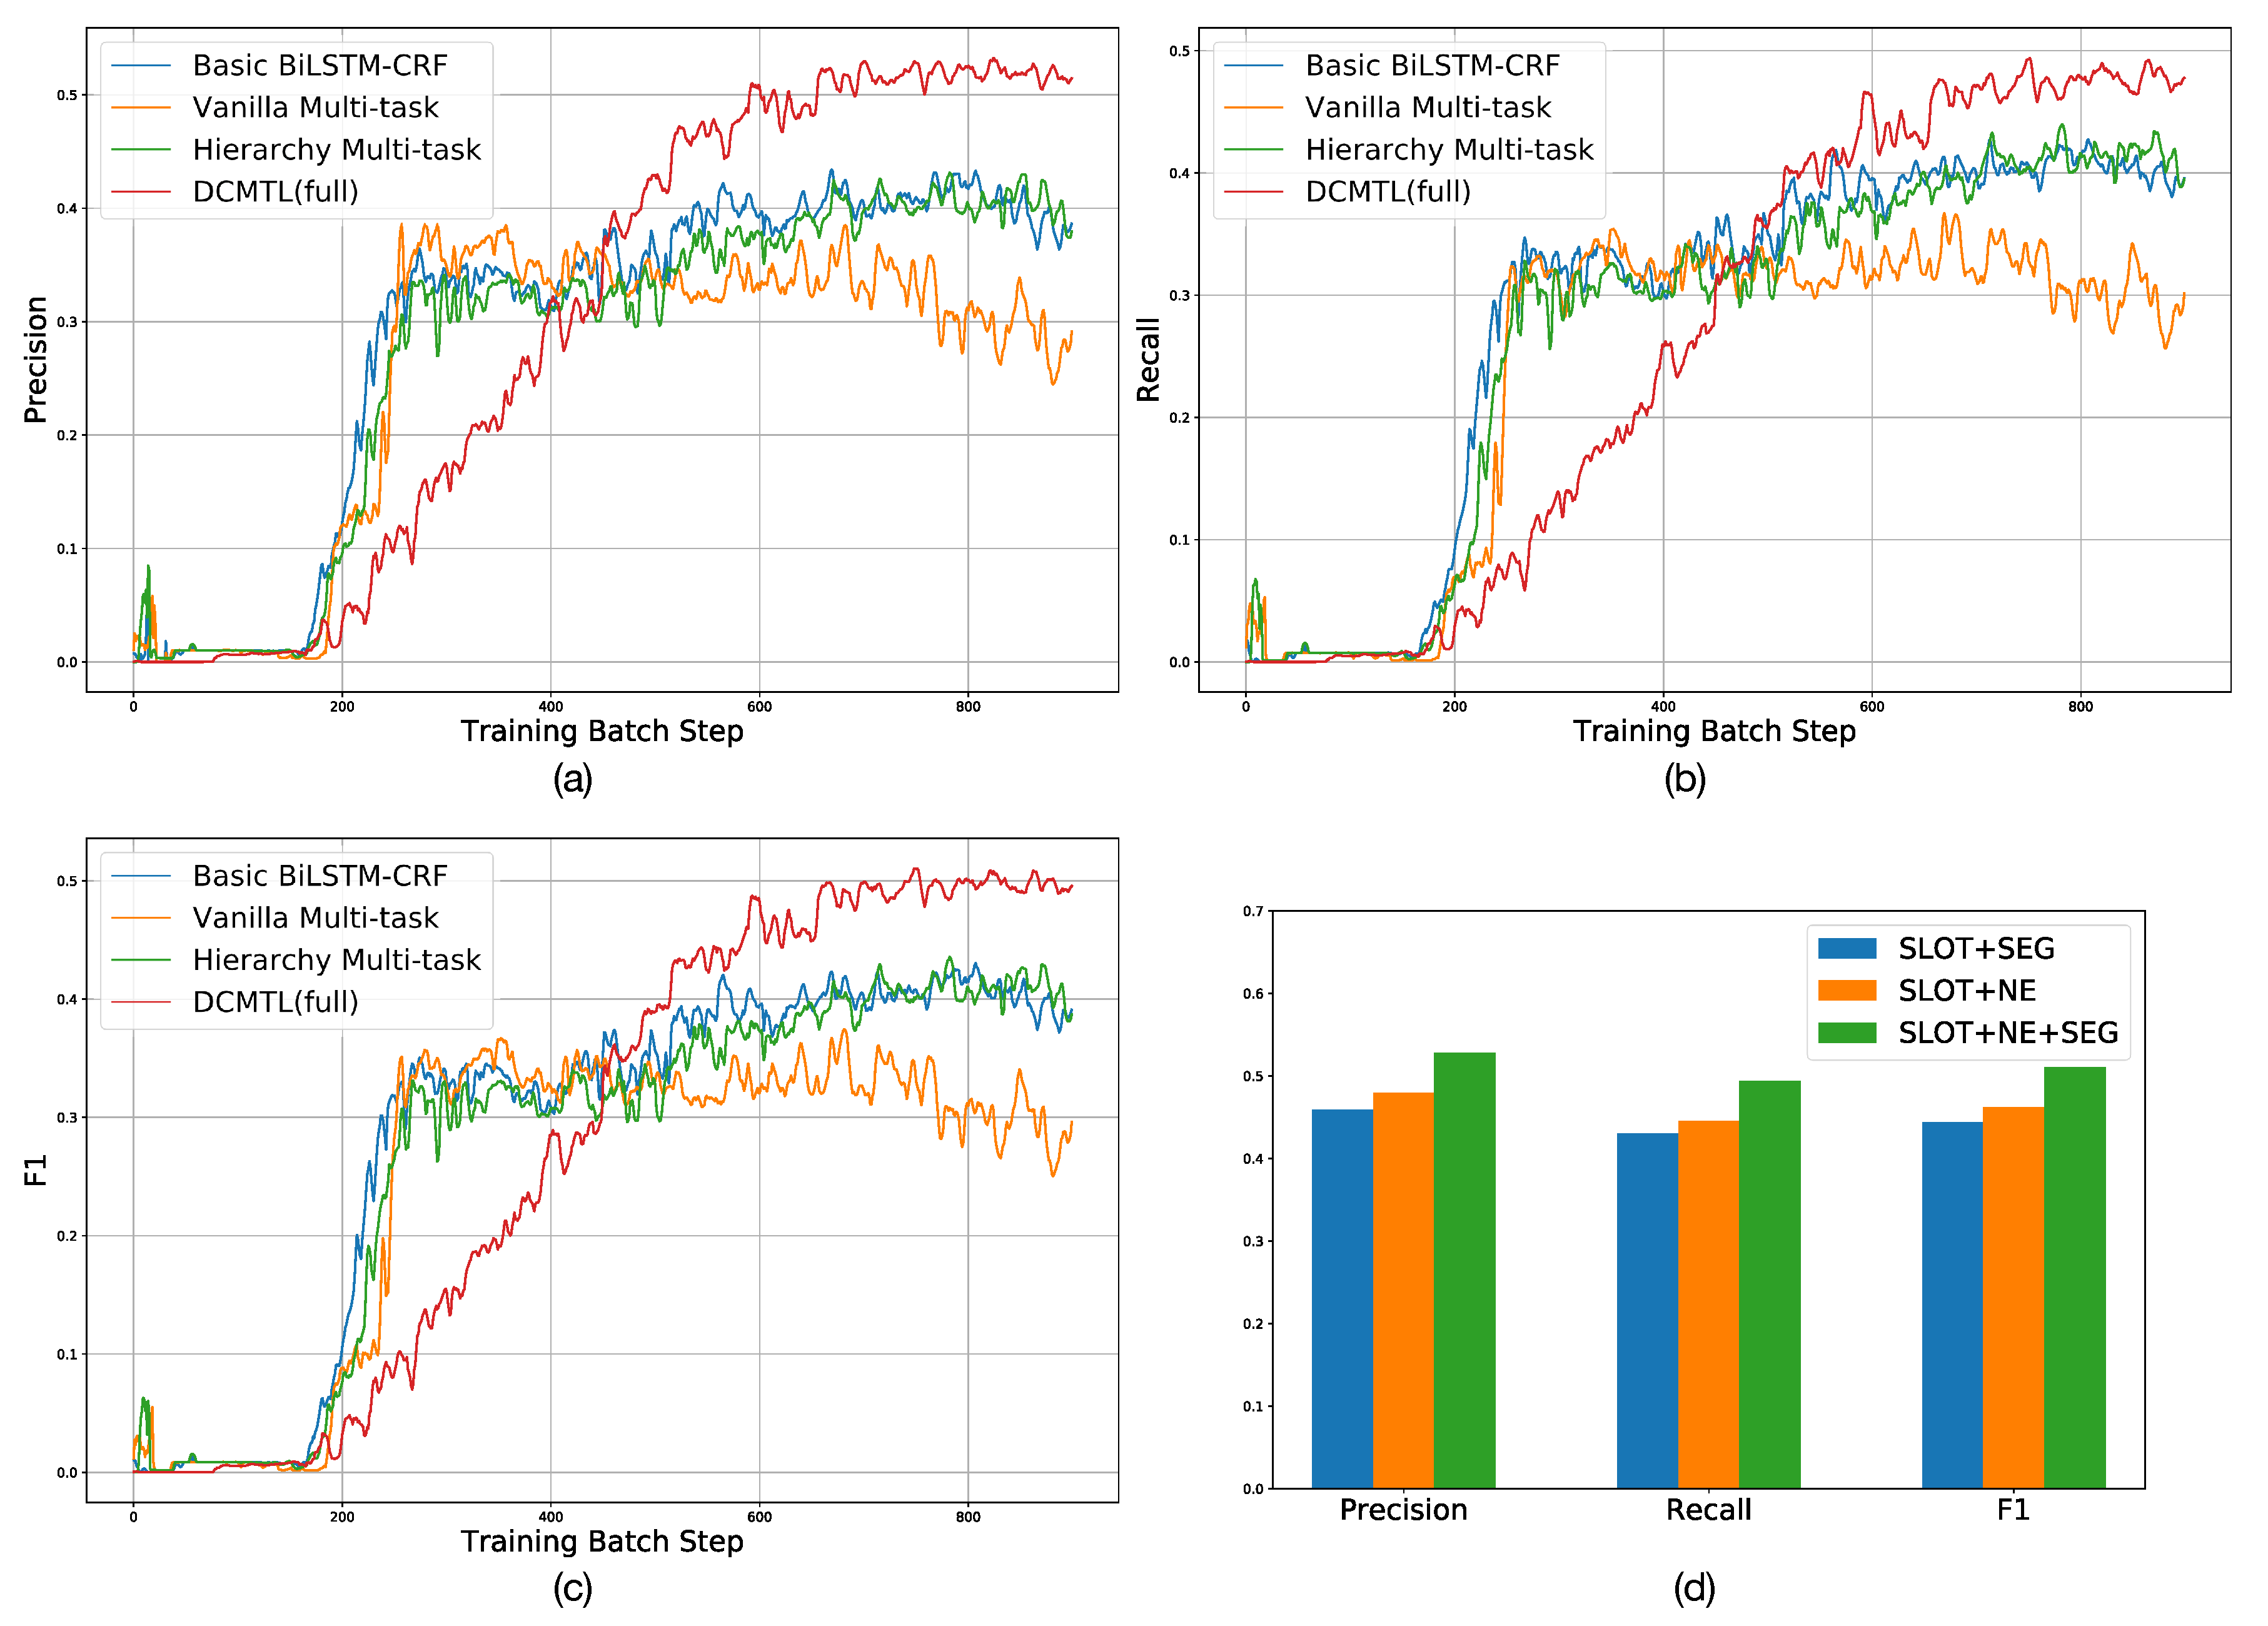
\epsfig{file=figures/learning_curve.eps, width=1.0\columnwidth}
	%\subfigure[]{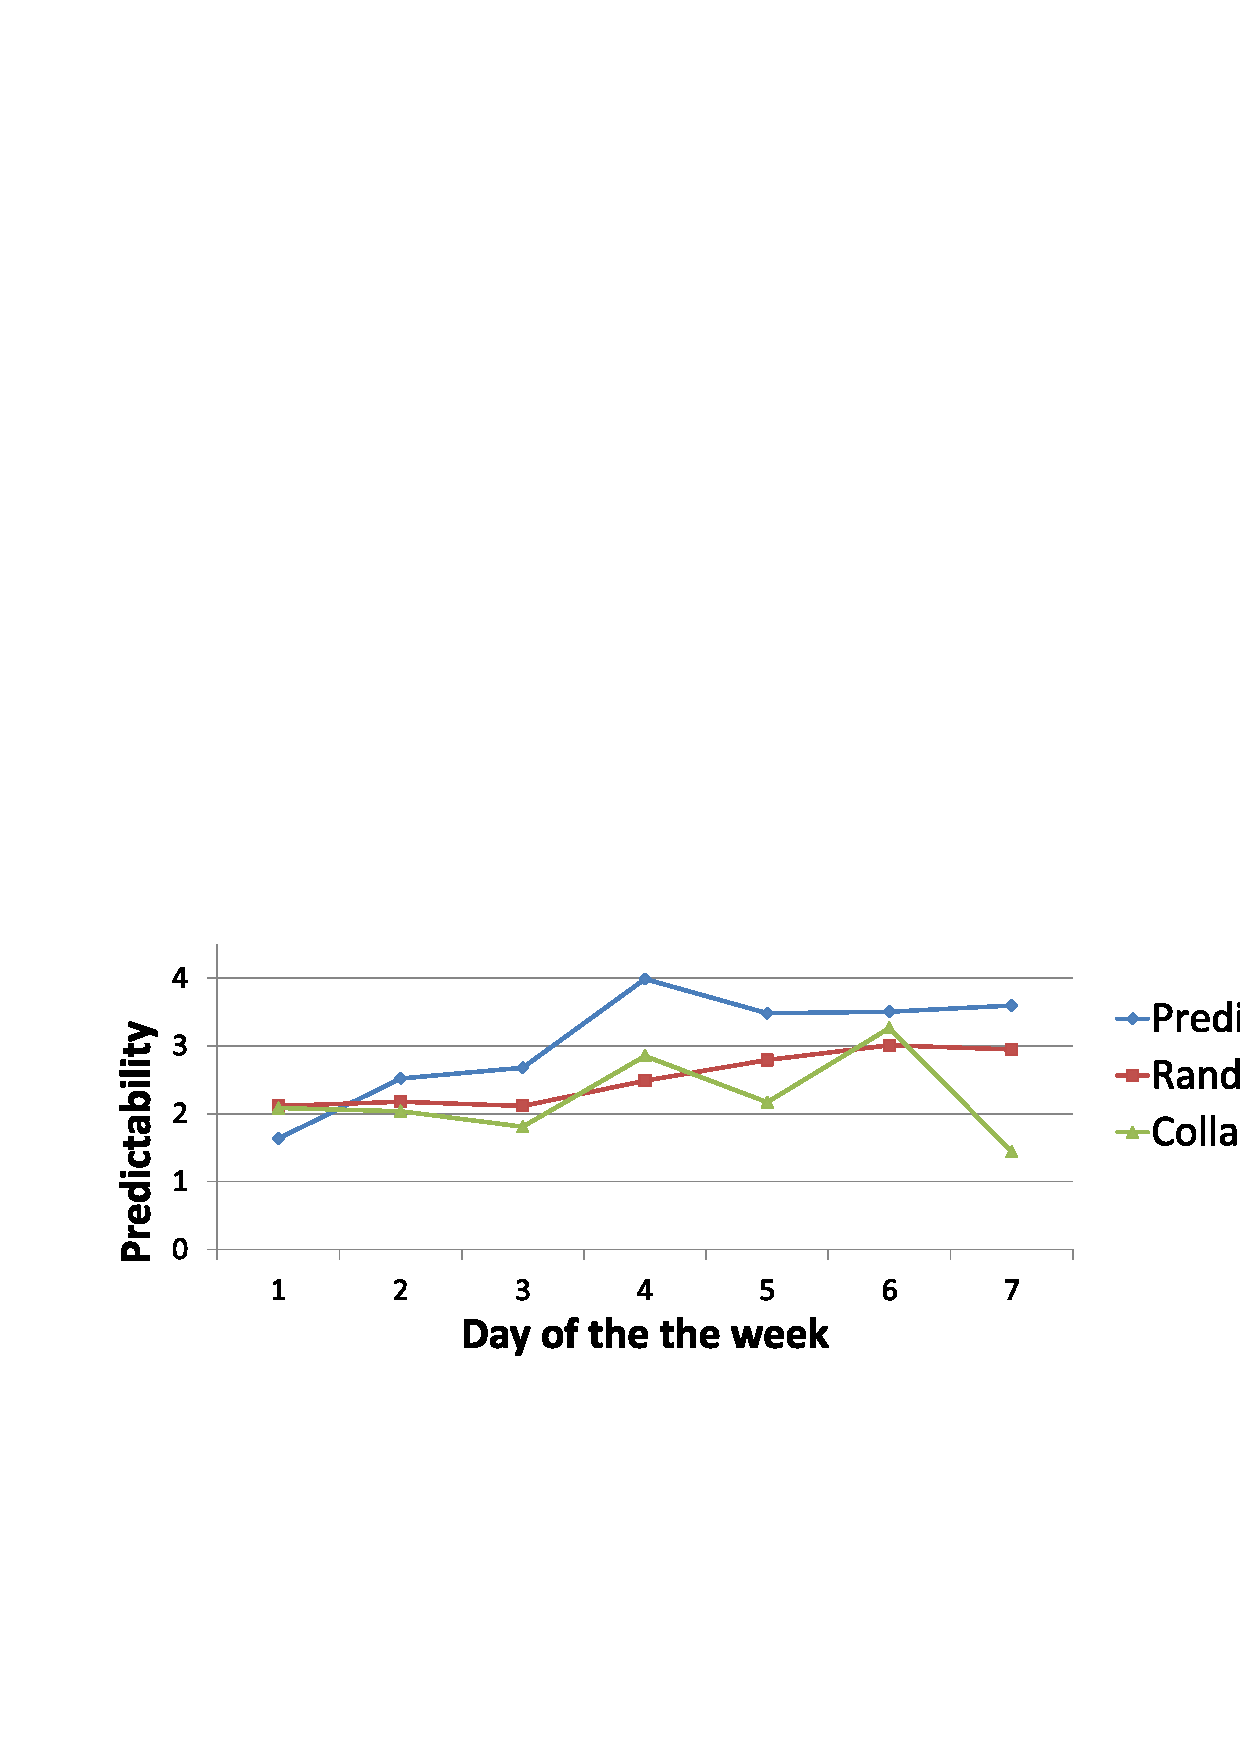
\includegraphics[width=0.65\columnwidth]{figures/precision.pdf}}
	%\subfigure[]{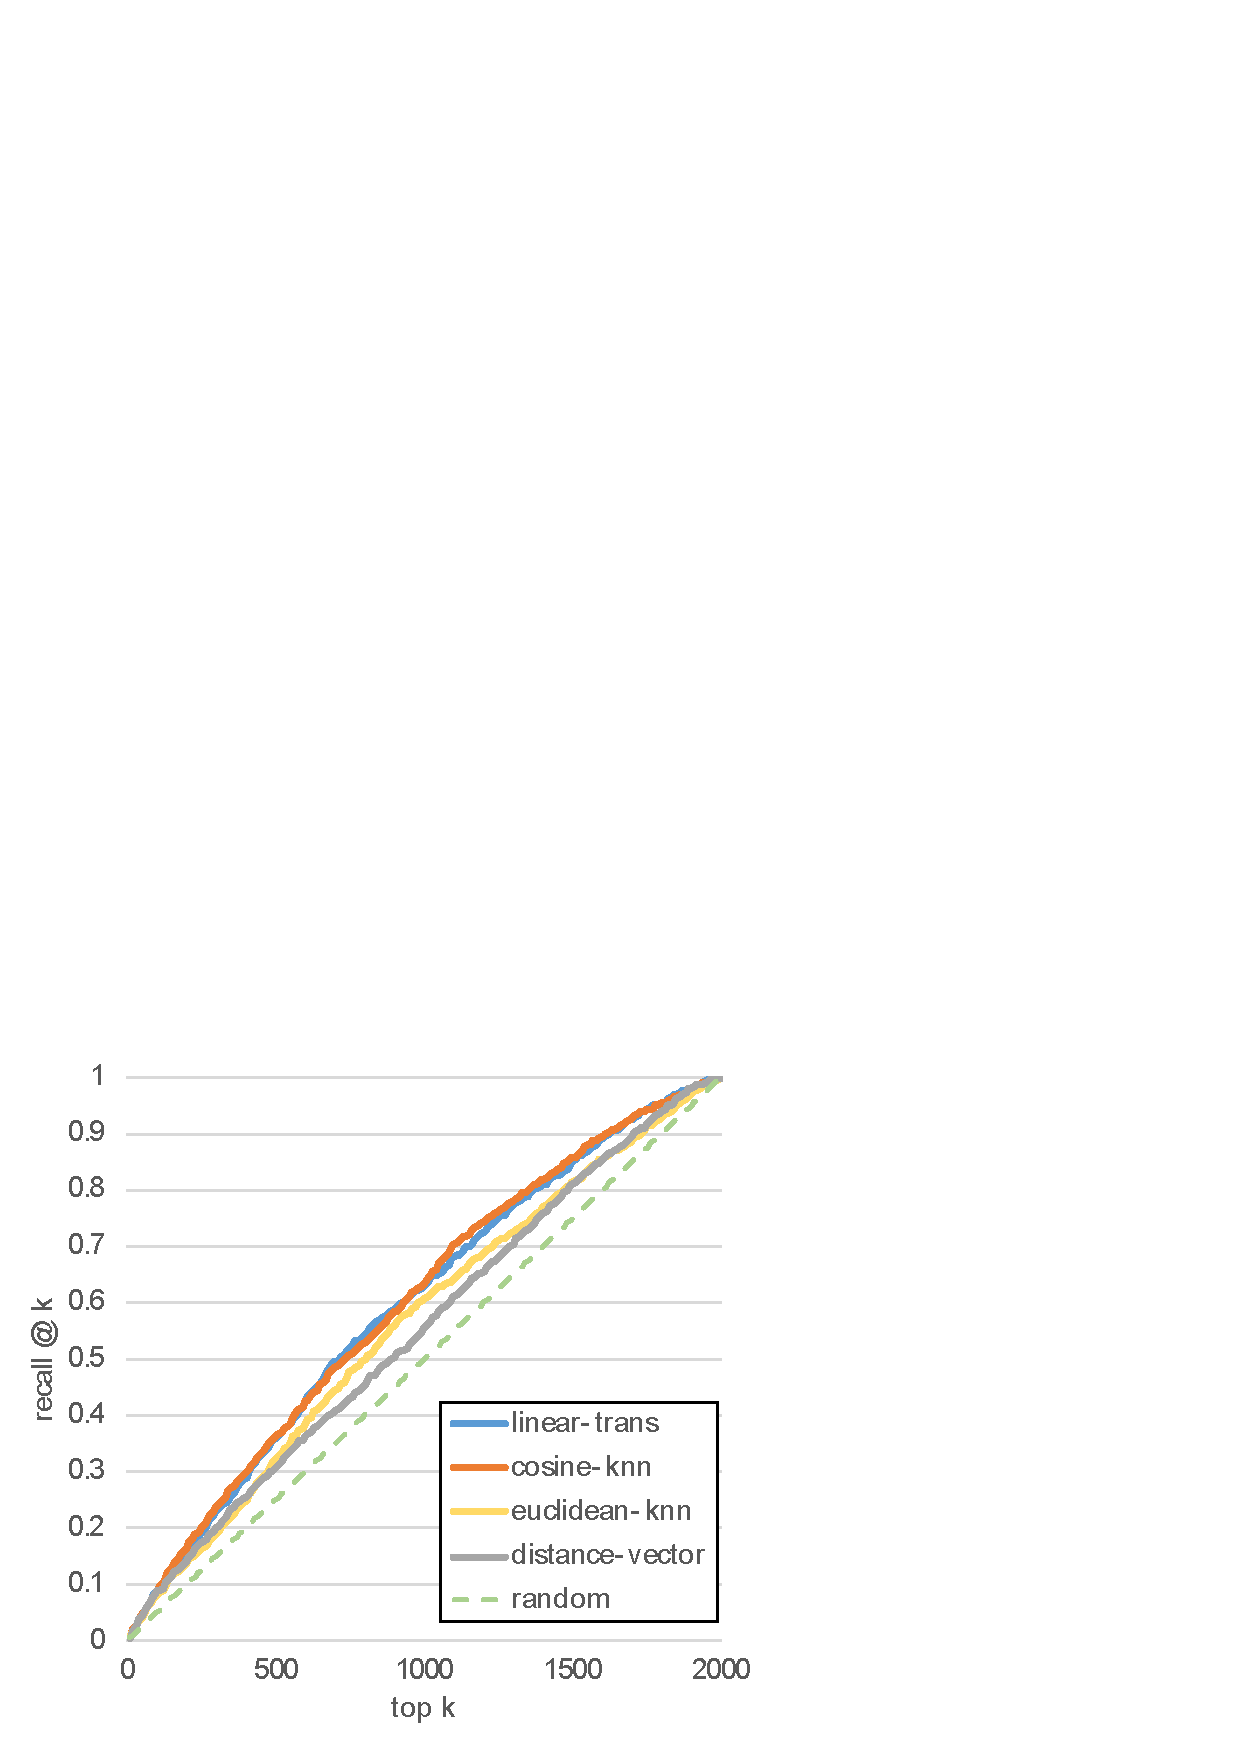
\includegraphics[width=0.65\columnwidth]{figures/recall.pdf}}
	\subfigure[]{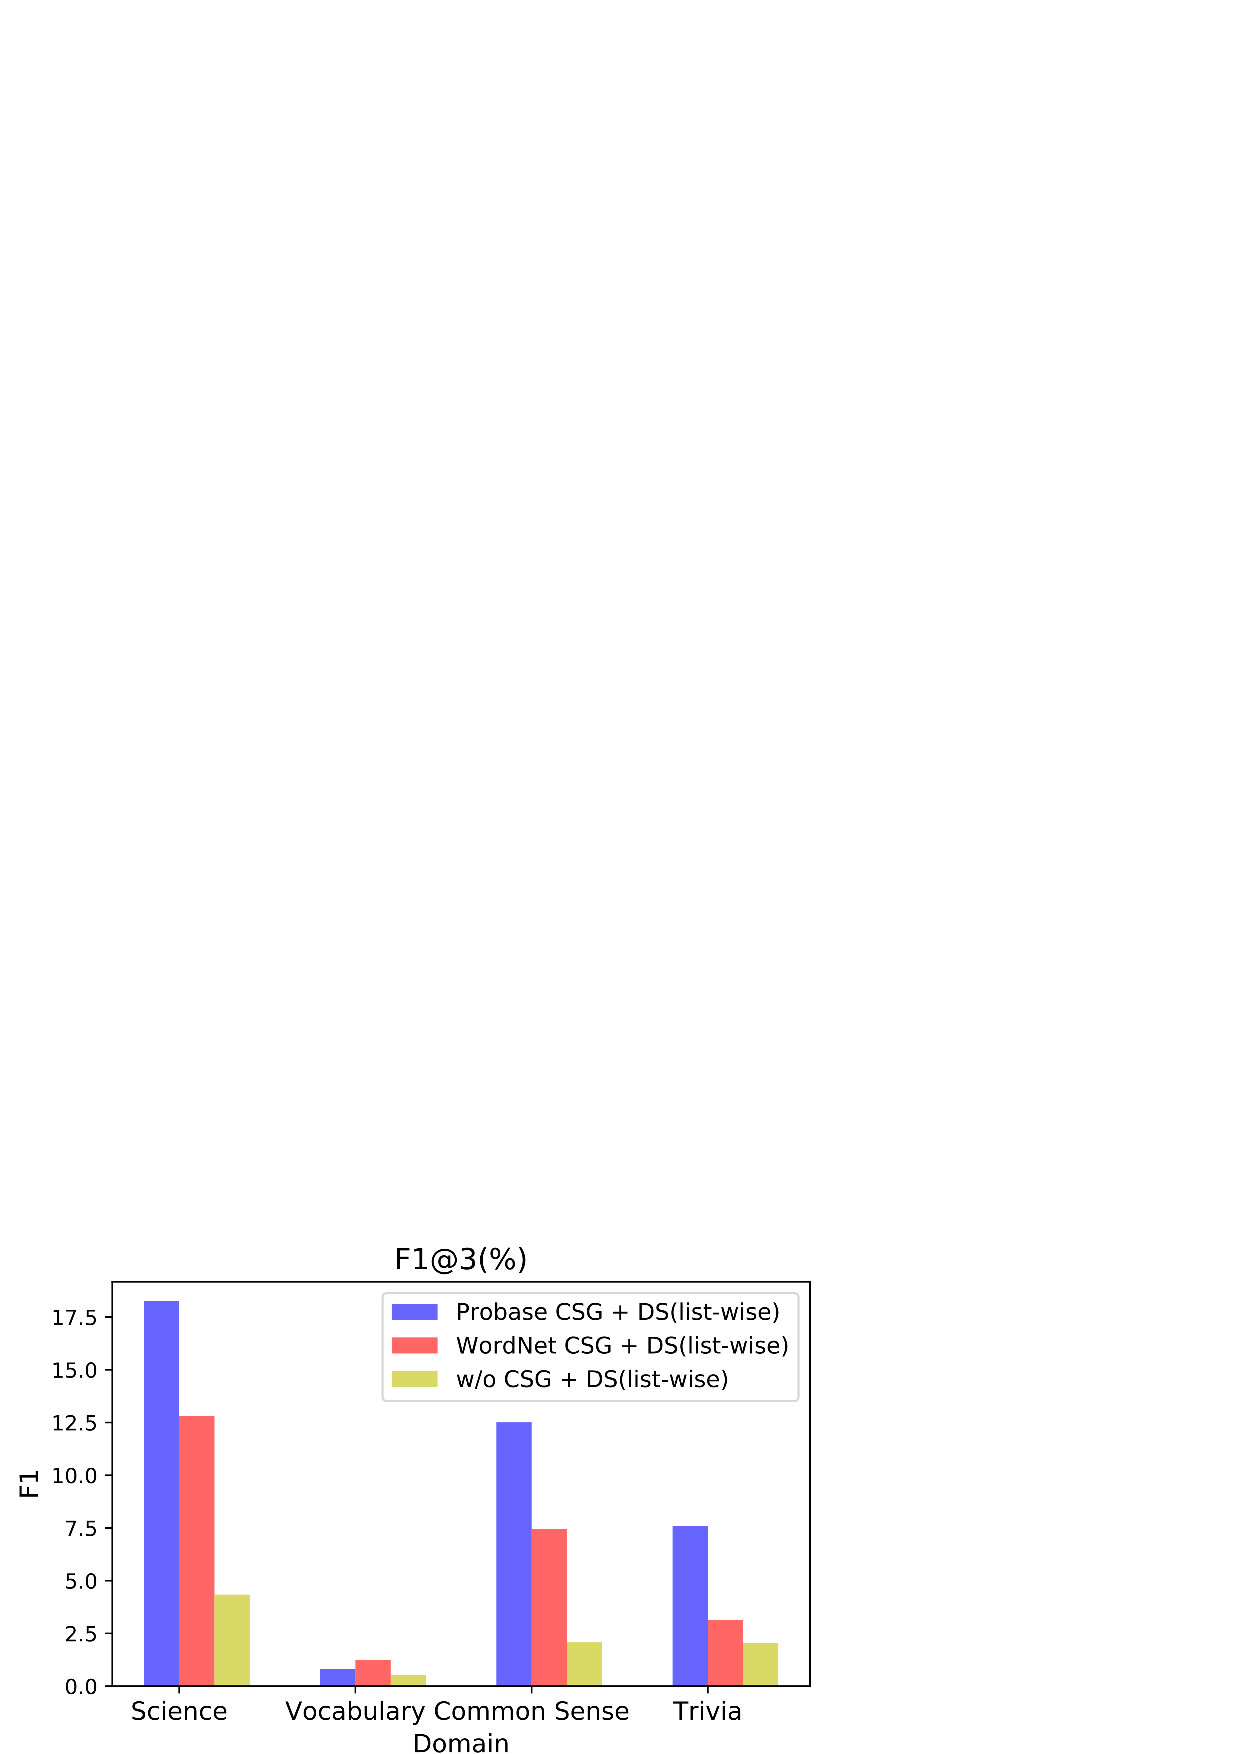
\includegraphics[width=0.49\columnwidth]{figures/f1.pdf}}
	\subfigure[]{\includegraphics[width=0.49\columnwidth]{figures/multi_grained.pdf}}
	\caption{(a) Learning trends of F1 respectively for different methods.
	(b) Result of different cascade connection types in DCMTL.}
	\label{fig:learning_curve}
	%\vspace{-10pt}
\end{figure}

On ECSA dataset,
we evaluate different models including 
Basic BiLSTM-CRF, Vanilla Multi-task, 
Hierarchy Multi-task and Deep Cascade Multi-task
on testing data regarding slot filling as the target task. %\yu{Should cite?}
We report Precision, Recall and F1 in \tabref{tab:eval_ECSGA}.

The Basic BiLSTM-CRF model achieves an F1 score of 0.43.
To show the usefulness of the lower tasks to slot filling,
we ``cheated'' by using the ground-truth segment type (cond. SEG) or 
named entity type (cond. NE) as the extra features for each word
in the Basic BiLSTM-CRF model.
Row 3 and 4 (with *) in \tabref{tab:eval_ECSGA} show that the slot filling 
performance can be improved by 85\% and 109\% if the correct segment type
or named entity type is pre-known.
It can perfectly verify our claim that low-level syntactic tasks can significantly affect to the slot filling performance.
Of course in practice, the model doesn't know the true values of these types during prediction.
%\KZ{The above to show an upper bound right? Need to point this out.}

Our further experiments show that DCMTL outperforms the 
baselines on both precision and recall.
DCMTL achieves the best F1 score of 0.5105, 
which improves by a relative margin of 14.6\% 
against the strong baseline method (see \tabref{tab:eval_ECSGA}).
Multi-task models generally perform better than the Basic 
BiLSTM with single-task target.
The exception is the vanilla multi-task setting.
This is mainly because 
vanilla multi-task shares parameters across all the layers,
and these parameters are likely to be disturbed by the interaction of 
three tasks. It is more desirable to let the target task dominate the 
weights at high-level layers.
%From the loss 
%$L=\alpha L^{seg}+\beta L^{ner}+(1-\alpha-\beta)L^{slot}$ (\secref{sec:training}),
%hyper-parameters $\alpha$ and $\beta$ significantly affects 
%the performance. 
%If we can not tune them perfectly 
%(we just set defaulted $\alpha=\beta=1/3$ in this experiment),
%the target task will suffer from the additional noise a lot.

We further investigate the learning trend of our proposed approach against baseline methods.
\figref{fig:learning_curve}(a) shows the typical learning curves 
of performance measured by F1.
We can observe that our method DCMTL 
performs worse than other baseline methods
for the first $450$ batch steps.
After that, other methods converge quickly 
and DCMTL perform much better after $500$ batch steps
and finally converge to the best F1 score.
We believe that in the beginning,
high-level task in DCMTL is affected more by the noise of low-level tasks comparing to others,
but as the training goes on,
the high-level slot filling task slowly reaps the benefits from low-level tasks.
%\yu{Another explanation is that the convergence for the DCMTL has been
%	delayed thus it had the opportunity to explore more areas and achieves better
%	results.}

%{\color{red}[[Modification Start]]}
To make our experiments more solid, 
we implemented two previous best performing models on ATIS dataset: 
Sequential CNN \cite{vu2016sequential} (Sequence Labeling based) and Neural Sequence Chunking \cite{zhai2017neural} (Encoder-Decoder based).
They achieved 0.2877 and 0.4355 F1 scores respectively, while
our DCMTL model scores 0.5105 F1 and outperforms both of them (by \textbf{77\%} and \textbf{17\%} improvements).
%One possible reason is that they never use any sequential output methods (e.g. CRF).
%It is not a problem on ATIS dataset with fewer chunked words but 
%their performance is seriously affected when testing on ECSA dataset
%which has much richer expressions.
%\yu{I wonder if reviewers will argue about it.}
%{\color{red}[[Modification End]]}
%\begin{table}[th]
%	\centering
%	\scriptsize
%	\begin{tabular}{c|c|c|c}
%		\toprule
%		Methods & Sequential CNN & Neural Sequence Chunking & DCMTL \\
%		\midrule
%		F1 &  &  & \textbf{0.5105} \\
%		\bottomrule
%	\end{tabular}
%	\caption{Comparison with published results on the ECSGA dataset.}
%	\label{tab:eval_ECSGA_SOTA}
%	\vspace{-10pt}
%\end{table}

%\noindent
\subsubsection{Ablation Test}
Our ``shortcuts'' connections come in two flavors: cascade connection and residual connection.
Multi-task outputs and ``shortcuts'' connections are highly related since without the multi-task framework, there will be no cascade connections.
We go on to show that both multi-task setting and the ``shortcuts'' connections are effective and useful in \tabref{tab:eval_ECSGA},
where F1 score improves from 0.4302 to 0.4455 and 0.5105 respectively.
We also investigate how our model DCMTL performs with or without cascade and residual connections (rows with ** prefix in \tabref{tab:eval_ECSGA}).
F1 score increases from 0.4840 to 0.5105 when residual connection is applied, which verifies its benefit.
If we remove cascade connection from DCMTL,
the model actually degenerates into hierarchy multi-task model with residual connection and performs 0.4633 F1 score.
Thus we can conclude that both connections are helpful for our DCMTL model.
However, the cascade connection, which relies on the multi-task, is more effective than the residual connection.
We can verify it from the fact that DCMTL model without cascade connection performs much worse than without residual connection (0.4633 vs. 0.4840 F1 scores).

Furthermore, 
we explore how DCMTL performs with different cascade connection methods.
We compare three different types of cascade connection 
illustrated in \figref{fig:cascade_connection_type}(a):
\begin{enumerate}
\item[1.]
	Segment labeling skipped to slot filling (SLOT+SEG).
\item[2.]
	Named entity labeling directly connected to slot filling \\(SLOT+NE).
\item[3.]
	Segment labeling, named entity labeling and slot filling in sequence (SLOT+NE+SEG).
\end{enumerate}

From \figref{fig:learning_curve}(b),
we find that cascade connection with type 3 
performs the best
and then with type 2,
while cascade method with skipped connection (type 1) performs the worst.
Therefore, we design the networks 
with a cascade connection in a hierarchical fashion
and do not apply skipped connection for the cascade 
inputs (\figref{fig:cascade_connection_type}(b)).
%\KZ{Can you speculate why type 3 and 2 are better than 1?}
This phenomenon here may also be proved by our ``cheated'' case study above.
Slot filling performance with pre-known named entity type is 
much better than with pre-known segment type
(rows with * in \tabref{tab:eval_ECSGA}).
\begin{figure}[h]
	\centering
	\subfigure[]{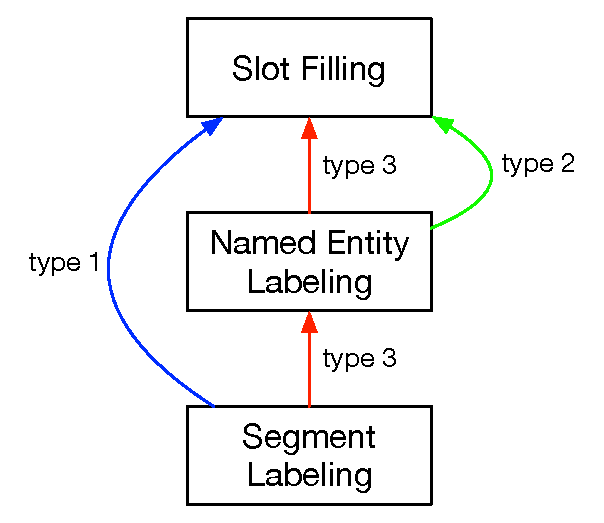
\includegraphics[width=0.48\columnwidth]{figures/cascade_connection_show.eps}}
	\subfigure[]{\includegraphics[width=0.48\columnwidth]{figures/cascade_connection_type.eps}}
	\caption{(a) Three types of cascade connection in our experiment.
		(b) Comparison between hierarchical and skipped cascade connection.}
	\label{fig:cascade_connection_type}
	%\vspace{-10pt}
\end{figure}
%\begin{figure}[h]
%	\centering
%	\epsfig{file=figures/multi_grained.pdf, width=0.8\columnwidth}
%	\caption{Results of different cascade connection types in DCMTL.}
%	\label{fig:multi_grained}
%	\vspace{-10pt}
%\end{figure}

\subsection{Online Testing}
\label{sec:case_study}
%We deployed DCMTL and baseline method (BiLSTM-CRF) on the online 
%operational Taobao Shopping Assistant system and analyzed the users query log.
%Take the slot label result of term ``一字领 (boat neckline)'' as 
%an example (\tabref{tab:case_study}).
%DCMTL regards the whole trunk as Neckline Style,
%while the baseline method splits it into two trunks (``一字'' and ``领'') and label ``一字'' as Contour Style.
%We believe the reason is that if we do not know the segment information
%then the prediction of slot label may be disturbed by some similar terms such as ``A字 (A-line)'' which is Contour Style.
Previous experimental results have proven the advantages of
our proposed DCMTL approach, so we deploy it in a real
world online environment to test its practical performance.

For online A/B testing, we extracted users query log with the slot filling results for one day. There are in total 251,409 unique queries.
We let three persons to manually evaluate whether a query is slotted perfectly with the strategy where the minority obeys the majority.
A query is slotted perfectly means all terms in query are assigned with the correct slot labels.
Our DCMTL model results in 152,178 perfectly slotted queries which is \textbf{60.53\%} accuracy\footnote{We only report accuracy as evaluation metric, because precision and recall are the same in such case.}.
While the original online max-matching algorithm with E-commerce knowledge base\footnote{As we have showed that our DCMTL model outperforms several strong baselines in the offline evaluation, and the gap between online and offline is minor since our offline dataset also comes from online queries, 
we only deploy DCMTL model online since such evaluation is costly.} 
(more details in \secref{sec:ECSGA_data})
only covers 66,302 perfectly slotted queries with \textbf{26.37\%} accuracy.
Thus, 
the accuracy of query slot filling in such online shopping assistant 
system is improved by 130\% after deploying DCMTL model.
This demonstrates that our model can effectively
extract the semantic attributes of users query which is extremely helpful E-commerce Shopping Assistant system.

%to guarantee the user experience of product searching.

%\begin{table}[h]
%	\centering
%	\scriptsize
%	\caption{Case study for term ``一字领 (boat neckline)'' in online query.
%		In slot labels, \textbf{NS} is short for \textbf{Neckline\_Style}
%		and \textbf{CS} is short for \textbf{Contour\_Style}.}
%	\begin{tabular}{c|c|c|c|c}
%		\toprule
%		\multicolumn{2}{c|}{\multirow{2}{*}{Term}} & 一 & 字 & 领  \\
%		\cmidrule{3-5}
%		\multicolumn{2}{c|}{} & \multicolumn{3}{c}{\emph{boat neckline}} \\
%		\midrule
%		\multirow{2}{*}{DCMTL} & Segment Label & \textbf{B} & \textbf{I} & \textbf{I} \\
%		\cmidrule{2-5}
%		& Slot Label & \textbf{B-NS} & \textbf{I-NS} & \textbf{I-NS} \\
%		\midrule
%	 	\multirow{2}{*}{Baseline} & Segment Label & \textbf{B} & \textbf{I} & \textbf{B} \\
%		\cmidrule{2-5}
%		& Slot Label & \textbf{B-CS} & \textbf{I-CS} & \textbf{B-NS} \\
%		\bottomrule
%	\end{tabular}
%	\label{tab:case_study}
%	\vspace{-10pt}
%\end{table}

%We also extracted the terms in online queries which are slotted as \textbf{Neckline\_Style} and \textbf{Material} by DCMTL as show cases (\tabref{tab:show_case}).
%We can see that online user utterances are much more complicated and contain 
%lots of synonyms or aliases. For example, ``纯棉/棉质/棉布/全棉/棉/绵绸'' all mean \emph{cotton}.
%
%\begin{table}[h]
%	\centering
%	\scriptsize
%	\caption{Example terms slotted as \textbf{Neckline\_Style} and \textbf{Material}.}
%	\begin{tabular}{|l|}
%		\hline
%			\large{\textbf{Neckline\_Style}} \\
%		\hline
%			保罗领 (Polo neckline) / 一字领 (boat neckline) / 翻领 (lapel)\\
%			衬衫领 (shirt collar) / V字领 (V-neck) / 深V领 (deep V-neck) \\
%			圆领 (round collar) / 立领 (stand collar)  \\
%			荷叶边领 (lotus leaf collar) / 方口领 (square collar) \\
%			水滴领 (drop collar) / 复古领 (vintage collar) / 半领 (half collar) \\
%			飘带领 (floating collar) / 和服领 (kimono collar) \\
%			梯形领 (trapezoid collar) / 宽领 (wide collar) / 平领 (horizontal collar) \\
%			水手领 (sailor collar) / 珍珠领 (pearl collar) / 花领 (flower collar) \\
%			波浪领 (wave collar) / 尖领 (pointed collar) / 交叉领 (cross collar) \\
%			花瓣领 (petal collar) / 中式领 (chinese collar) \\
%			旗袍领 (Cheongsam collar) / 鸡心领 (sweetheart neckline)  \\
%		\hline
%		\hline
%			\large{\textbf{Material}} \\
%		\hline
%			棉麻 (cotton and linen) / 纯棉 (cotton) / 亚麻 (linen) \\
%			棉质 (cotton) / 棉布 (cotton) / 鹿皮绒 (suede) / 皮 (leather) \\
%			全棉 (cotton) / 毛线 (wool) / 天丝 (tencel) / 麻布 (linen) \\
%			冰麻 (ice linen) / 丝棉 (silk cotton) / 棉 (cotton) / 混纺 (blended) \\
%			麂皮 (suede) / 棉纱 (cotton yarn) / 桑蚕 (silkworm)  \\
%			pvc (pvc) / 木 (wood) / 丝光 (silk) / 纤维 (fiber) \\
%			绵绸 (cotton) / 鸵鸟毛 (ostrich feather) / 棉料 (cotton) / 银 (silver) \\
%			貂绒 (velvet) / 帆布 (canvas) / 皮质 (leather) / 棉线 (cotton thread) \\
%			塑料 (plastic) / 乳胶 (emulsion) / 毛绒 (Plush) / 棉花 (cotton) \\
%			莱卡 (lyca) / 皮绒 (leather) / 棉麻料 (cotton and linen) \\
%			绒布 (flannel) / 羽绒 (down) / 海绵 (sponge) / 尼龙 (nylon) \\
%			亚麻布 (linen) / 绢丝 (silk) / 山羊绒 (cashmere) / 橡胶 (rubber) \\
%			漆皮 (patent leather) / 冰丝 (Ice silk) / 羊毛绒 (wool velvet) \\
%		\hline
%	\end{tabular}
%	\label{tab:show_case}
%	\vspace{-10pt}
%\end{table}
